\chapter{Dicom-Presenter Rendering Engine}
\vspace{-10mm}
Dicom-Presenter as firstly designed in work \cite{neskudla} was an application depending on cca eight external libraries. The libraries dependency complicated application compilation and deployment. All the libraries must be executable on a target machine.

Therefore, a valuable task was to remove some of the library dependencies. Most of the deployment complications were related to OpenGL library. Besides OpenGL itself, GLEW, Cg toolkit and plib libraries were used to extend OpenGL functionality. All the libraries need to be hardware and software supported on the target machine\footnote{The OpenGL library requires GPU drivers supporting the library to be installed on the target machine. GLEW library require the GPU to support spatial textures (among others). Cg toolkit library requires the GPU to support pixel shader. Moreover, the Cg toolkit library requires a hardware-dependent configuration during the compilation time or at run time.}. Hence, removing OpenGL library with all three dependencies would contribute to application deployability.

The OpenGL library was connected to nine of all twenty-six Dicom-Presenter modules. Global OpenGL function were called within the modules considering previous OpenGL function calls done in another modules. Therefore, removing the OpenGL library from the application is a significant intervetion to the existing source code. To understand the new non-OpenGL implementation, it is mandatory to be familiar with application object model.

\section{Dicom-Presenter Object Model}

Dicom-Presenter consists of twenty six modules, together making 5000 lines. Each module includes one class (rarely two classes). The classes can be divided into two groups: classes which represent some visible element (image, workspace, ...) and classes which maintain only abstract functionality.

To understand the hierarchical arrangement of application classes, the following passages describes three views on the object model:

\begin{itemize}
\item Rendering the visual content. All the classes related to some visible element must be sequently called to paint their content to buffer container.
\item Control events forwarding. Each captured pointing device event must be forwarded to the object to which it belongs.
\item Image storing. A view on the object model related to the classes maintaining abstract functionalities can start with the actions attached to loading an image from hard disk.
\end{itemize}

\subsection{Dicom-Presenter Object Model Description}
As was said in \ref{dicom-presenter}, Dicom-Presenter application window consists of:  Workspace, Image Explorer, Workspace Explorer and Info Panel. The Workspace act as a main graphic output, it is used for viewing DICOM images. To ensure usability of Dicom-Presenter during presentations, several workspace sessions can be opened at the same time. Therefore, Workspace Explorer acts as a switch among opened workspaces\footnote{The process is similar as workspaces switching in GNOME/KDE.}. Since an image can be opened at a number of workspaces at once, Image Explorer is used to manage opened images. Info Panel holds information about the opened image or the opened workspace.

\subsection{Graphic Output Rendering in Dicom-Presenter}
The mentioned control elements of Dicom-Presenter: Image Explorer and Workspace Explorer are rendered manually. They are not based on existing Qt library class. Thus, if a graphic output of Dicom-Presenter is rendered all classes representing some graphic element must be called. 

An impulse to render the graphic window can be called at any time from any part of the application. A static function is used to obtain the pointer to output window, then a function called \clist{paint} is called.

The \clist{paint} function of main window object (\clist{CWidget}) then calls paint functions of all elements present in the window: an active Workspace, Workspace Explorer and Image Explorer. All the elements contain smaller subelements. The Workspace calls paint functions of all images present appearing on the Workspace, Workspace Explorer calls paint functions of all images containing workspace previews and finally the Image Explorer calls paint functions of all images operated by it. A schema of the process can be seen on Figure \ref{paint}.

\begin{figure}
	\begin{center}
	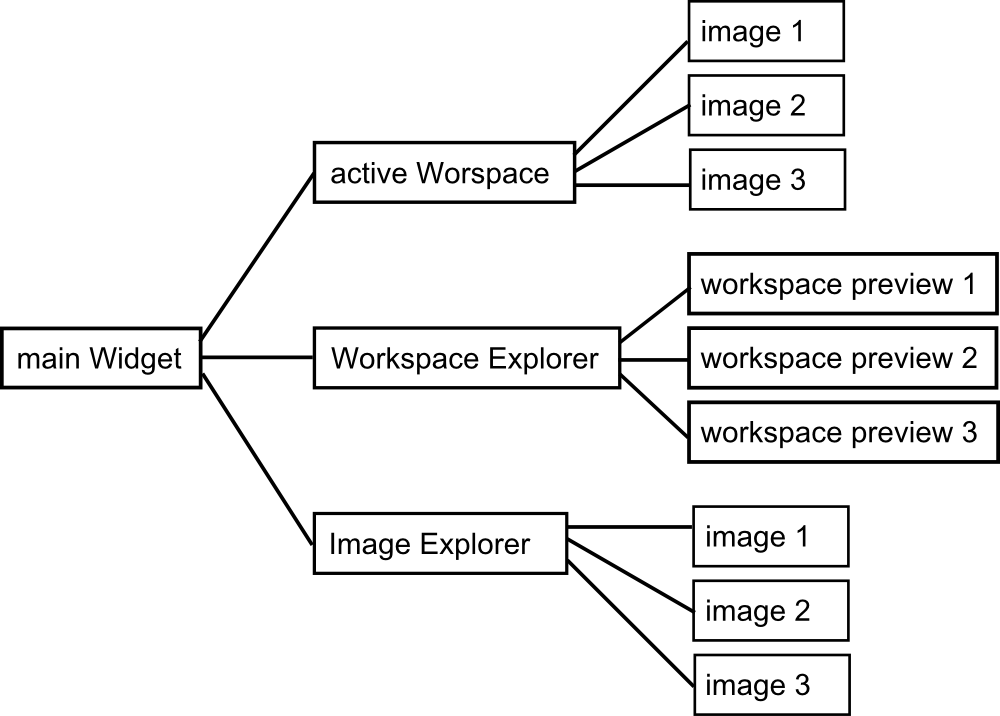
\includegraphics[width=130mm]{Text/IMG/paint.png}
	\end{center}
	\caption{A hierarchy of classes presenting paintable elements.}
	\label{paint}
\end{figure}

\subsection{Control Event Forwarding in Dicom-Presenter}

\subsection{Image Opening in Dicom-Presenter}





\section{Rendering Engine Implementation}
\red{podrobne rozepsat, jake tridy byly pouzity a co delaji}